% \documentclass[12pt, twoside]{article}
\usepackage[letterpaper, margin=1in, headsep=0.2in]{geometry}
\setlength{\headheight}{0.6in}
%\usepackage[english]{babel}
\usepackage[utf8]{inputenc}
\usepackage{microtype}
\usepackage{amsmath}
\usepackage{amssymb}
%\usepackage{amsfonts}
\usepackage[nomessages]{fp} %\FPeval{\var-name}{2*sin(pi/6)}
\usepackage{siunitx} %units in math. eg 20\milli\meter
\usepackage{yhmath} % for arcs, overparenth command
\usepackage{tikz} %graphics
\usetikzlibrary{quotes, angles, arrows, arrows.meta}
\usepackage{graphicx} %consider setting \graphicspath{{images/}}
\usepackage{parskip} %no paragraph indent
\usepackage{enumitem}
\usepackage{multicol}
\usepackage{venndiagram}

\usepackage{fancyhdr}
\pagestyle{fancy}
\fancyhf{}
\renewcommand{\headrulewidth}{0pt} % disable the underline of the header
\raggedbottom
\hfuzz=2mm %suppresses overfull box warnings

\usepackage{hyperref}

\fancyhead[LE]{\thepage}
\fancyhead[RO]{\thepage \\ Name: \hspace{4cm} \,\\}
\fancyhead[LO]{BECA / Dr. Huson / Geometry\\*  Unit 3: Parallel lines and transversals\\* 27 October 2022}

\begin{document}

\subsubsection*{3.7 Review: Parallel lines, transversals, triangles mixed practice}
\begin{enumerate}
\item Identify the relationships among the angles made by two parallel lines and a transversal, as shown. True or False:
\begin{multicols}{2}
  \begin{enumerate}
    \item T \hspace{0.5cm} F \hspace{1cm} $\angle 3 \cong \angle 6$
    \item T \hspace{0.5cm} F \hspace{1cm} $\angle 4 \cong \angle 7$
    \item T \hspace{0.5cm} F \hspace{1cm} $m\angle 3 + m\angle 5 =  180$
    \item T \hspace{0.5cm} F \hspace{1cm} $m\angle 1 + m\angle 8 =  180$
  \end{enumerate}
    \begin{tikzpicture}[scale=0.7]
    \draw [<->, thick] (3,2)--(8,2);
    \draw [<->, thick] (2,0)--(7,0);
    \draw [<->, thick] (4,-1)--(5.5,3);
    \node at (4.5,0.3) [left]{$5$};
    \node at (4.5,0.3) [right]{$6$};
    \node at (4.3,-0.3) [left]{$7$};
    \node at (4.3,-0.3) [right]{$8$};
    \node at (5.2,2) [above left]{$1$};
    \node at (5.2,2) [above right]{$2$};
    \node at (5,2) [below left]{$3$};
    \node at (5,2) [below right]{$4$};
  \end{tikzpicture}
\end{multicols}

\item Find $m\angle 1$ given two parallel lines and a transversal, with
  \begin{multicols}{2}
  $\displaystyle m\angle 3 = 5x+21$ \hspace{0.75cm}$\displaystyle m\angle 5 = 9x-9$
  \begin{flushright}
  \begin{tikzpicture}[scale=1,rotate=-10]
    \draw [<->, thick] (3,2)--(8,2);
    \draw [<->, thick] (2,0)--(7,0);
    \draw [<->, thick] (4,-1)--(5.5,3);
    \node at (4.5,0.3) [left]{$5$};
    \node at (4.5,0.3) [right]{$6$};
    \node at (4.3,-0.3) [left]{$7$};
    \node at (4.3,-0.3) [right]{$8$};
    \node at (5.2,2) [above left]{$1$};
    \node at (5.4,2) [above right]{$2$};
    \node at (4.9,2) [below left]{$3$};
    \node at (5,2) [below right]{$4$};
  \end{tikzpicture}
  \end{flushright} 
  \end{multicols} \vspace{1cm}

\item Given two parallel lines, two transversals
  \begin{multicols}{2}
    \begin{enumerate}
      \item Find $x$, $y$
      \item What relationship are you using? \\[0.5cm]
      (e.g. vertical angles, corresponding angles, same-side exterior angles, alternate interior angles, etc.)
    \end{enumerate}
      \begin{tikzpicture}[scale=1.4]
      \draw [<->, thick] (4,2.25)--(7,2.25);
      \draw [<->, thick] (3.5,0)--(7,0);
      \draw [<->, thick] (4,-0.5)--(5.7,3);
      \draw [<->, thick] (6.5,-0.5)--(5,3);
      \node at (4.4,0.3) [right]{$69^\circ$};
      \node at (5.5,0.3) [right]{$86^\circ$};
      \node at (5.1,2.2) [below left]{$x$};
      \node at (5.5,2.2) [below right]{$y$};
    \end{tikzpicture}
  \end{multicols}
  
\item The measures in degrees of the three angles of a triangle are $2x$, $\frac{2}{5}x$, and $\frac{1}{10}x$. Find the measures of the triangle's angles. \vspace{4cm}

\newpage
\item Given  $\triangle LMN$ with $m\angle L=2x+20$, $m\angle N=3x+5$, and $m\angle M=5x+5$. Find $x$.
  \begin{flushright}
  \begin{tikzpicture}[scale=0.8]
    %\draw [->, thick] (0,0)--(5,5);
    \draw [-, thick] (0,0) node[below]{$L$}--
      (2.5,3) node[above]{$M$}--
      (5,0) node[below]{$N$}--cycle;
  \end{tikzpicture}
  \end{flushright} \vspace{2cm}

\item Given $\triangle RSU$. If $m\angle UST=x+50$, $m\angle R=x-20$, and $m\angle U=x+10$, find $m\angle R$.
  \begin{flushright}
  \begin{tikzpicture}[scale=0.8]
    %\draw [->, thick] (0,0)--(5,5);
    \draw [<-, thick] (8,0)--
      (7,0) node[below]{$T$}--
      (0,0) node[below]{$R$}--
      (2.5,3) node[above]{$U$}--
      (5,0) node[below]{$S$};
  \end{tikzpicture}
  \end{flushright} \vspace{3cm}

\item Angles $APC$ and $CPD$ form a linear pair. $m\angle APC = 10x+15$ and $m\angle CPD = 3x-4$. Find $m\angle CPD$. Check your answer for full credit.
  \begin{flushright}
    \begin{tikzpicture}[scale=0.8, rotate=-10]
      \draw [->, thick] (0,0)--(35:5);
      \draw [<->, thick] (-5,0)--(6,0);
      \draw [->, thick] (0,0)--(0,3);
      \draw (0,0)++(0.3,0)--++(0,0.3)--+(-0.3,0);
      %\draw [fill] (-1,2.5) circle [radius=0.05] node[left ]{$B$};
      \draw [fill] (35:4) circle [radius=0.05] node[below right]{$C$};
      \draw [fill] (-4,0) circle [radius=0.05] node[below]{$A$};
      \draw [fill] (0,0) circle [radius=0.05] node[below left]{$P$};
      \draw [fill] (0,2) circle [radius=0.05] node[left]{$B$};
      \draw [fill] (4,0) circle [radius=0.05] node[below]{$D$};
    \end{tikzpicture}
    \end{flushright}
    \vspace{4cm}

\newpage
\item Given two parallel lines that intersect a transversal,  $\overleftrightarrow{DE} || \overleftrightarrow{BC}$. $m\angle ABC =3x-5$ and $m\angle BDE=6x+5$. \par \medskip
  Find $m\angle ADE$. \par \bigskip
    \begin{tikzpicture}[scale=1.1]
      \draw [<->, thick] (-1,0)--(0,0)--(4,0);
      \draw [<->, thick] (-0.5,-0.5)--(3,3)--(3.5,3.5);
      \draw [<->, thick] (1,2)--(5, 2)--(5.5,2);
      \draw [fill] (3,3) circle [radius=0.05] node[above left]{$A$};
      \draw [fill] (5, 2) circle [radius=0.05] node[below]{$E$};
      \draw [fill] (2,2) circle [radius=0.05] node[above left]{$D$};
      \draw [fill] (0,0) circle [radius=0.05] node[above left]{$B$};
      \draw [fill] (3,0) circle [radius=0.05] node[below]{$C$};
    \end{tikzpicture} \vspace{3cm}

\subsubsection*{Do Not Solve}
\item Given two parallel lines and a transversal, with alternate interior angles $m\angle 4 = 5x$ and $m\angle 5 = 2x + 40$. Write an equation, to solve for $x$, but do not solve it. %Write an equation, then solve for $x$.
\begin{flushright}
  \begin{tikzpicture}[scale=1]
    \draw [<->, thick] (0,0)--(7,0);
    \draw [<->, thick] (1,2)--(8,2);
    \draw [<->, thick] (5,-1)--(3,3);
    %\draw [<->, thick] (11,-1)--(9,3);
    %\node at (4, 1.7){$1$};
    \node at (5, 2)[below]{$m\angle 4 = 5x$};
    \node at (4, 0)[above left]{$m\angle 5 = 2x + 40$};
    %\node at (10, 0.25){$3$};
  \end{tikzpicture}
  \end{flushright}

\item Two parallel lines intersect a transversal, shown. Given the same-side interior angles  $m\angle 4 = 16x - 79$ and $m\angle 6 = 6x + 50$. Write an equation, but do not solve it. %Solve for $x$ then find the measure of $\angle 4$. 
  \begin{flushright}
    \begin{tikzpicture}[scale=1]
      \draw [<->, thick] (3,0)--(9,0);
      \draw [<->, thick] (2,2)--(8,2);
      \draw [<->, thick] (5,-1)--(3,3);
      %\draw [<->, thick] (11,-1)--(9,3);
      %\node at (4, 1.7){$1$};
      \node at (5.5, 2)[below]{$m\angle 4 = 16x - 79$};
      \node at (6.2, 0.25){$m\angle 6 = 6x + 50$};
      %\node at (10, 0.25){$3$};
    \end{tikzpicture}
    \end{flushright}

\newpage
\item Given isosceles $\triangle LMN$, $\overline{LM} \cong \overline{NM}$. If $m\angle L=4x+19$ and $m\angle N=7x-8$, find $m\angle M$.
  \begin{flushright}
  \begin{tikzpicture}[scale=0.8]
    %\draw [->, thick] (0,0)--(5,5);
    \draw [-, thick] (0,0) node[below]{$L$}--
      (2.5,3) node[above]{$M$}--
      (5,0) node[below]{$N$}--cycle;
  \end{tikzpicture}
  \end{flushright} \vspace{2cm}

\item The measures in degrees of the three angles of a triangle are $3x$, $\frac{1}{2}x+7$, and $5x-65$. Find $x$. \vspace{3cm}

\item A triangle has two angles measuring $x^\circ$ and $y^\circ$ respectively. Find the measure of the third angle as an expression of $x$ and $y$. \vspace{3cm}

\item Given parallel lines $\overleftrightarrow{AB} \parallel \overleftrightarrow{CF}$, $m\angle BAE=75^\circ$ and $m\angle DAE=55^\circ$. \\[0.5cm]
  Find $m\angle ADC = x$ and $m\angle AEF = y$.
  \begin{flushright}
  \begin{tikzpicture}[scale=1.]
    \draw [<->, thick] (0,3)--(6.5,3) node[above left]{$B$};
    \draw [<->, thick] (-1,0) node[below right]{$C$}--
      (5,0)--
      (6,0) node[below left]{$F$};
    \draw [-, thick] (1,0) node[below]{$D$}--
      (2.5,3) node[above]{$A$}--
      (4.35,0) node[below]{$E$};
    \node at (2.6,2.4)[below]{$55^\circ$};
    \node at (2.9,2.8)[below right]{$75^\circ$};
    \node at (1,0)[above left]{$x$};
    \node at (4.4,0)[above right]{$y$};
  \end{tikzpicture}
  \end{flushright}


\end{enumerate}
\end{document}